\documentclass[aspectratio=169]{beamer}
\usepackage[utf8]{luainputenc}
\usepackage{amssymb,amsmath}
\usepackage{graphicx}
\usepackage{tikz}
\usepackage{beamercolorthemetud}
\usepackage[backend=biber]{biblatex}
\usepackage{caption}
\captionsetup[figure]{font=scriptsize}
\usepackage{hyperref}

\usepackage{subcaption}
\usepackage[absolute,overlay]{textpos}
  \setlength{\TPHorizModule}{1mm}
  \setlength{\TPVertModule}{1mm}




\addbibresource{bibl.bib}
\setbeamertemplate{bibliography item}{\insertbiblabel}
\usepackage[english]{babel}
\usetheme[]{tud}
\setbeamercolor{background canvas}{bg=}
\setbeamerfont{frametitle}{size=\Large}
\input{macros}



\title{MeetForSport: Adaptation Concept}
\author{Mattis Lahr, Felix Fischer}
\date{10.12.2021}

\einrichtung{\hspace{-1pt}Institute of Systems Architecture}
\datecity{Dresden}




\AtBeginSection[]{\partpage{\usebeamertemplate***{part page}}}
\begin{document}
\maketitle



\begin{frame}
    \frametitle{Table of Contents}
    \tableofcontents
\end{frame}



\section{App Idea}
\begin{frame}
\frametitle{MeetForSport}
This app will allow users to join group activities (i.e. football) or join ongoing events.
Targeting mostly active persons, this small social network will allow users  to find new friends/persons with the same interests and therefore allow these people to become more active.
\end{frame}

\section{Problematic Situations}
\begin{frame}   
	\frametitle{Situation 1:  Bad or no internet connection}
	 \begin{figure}
		\centering
		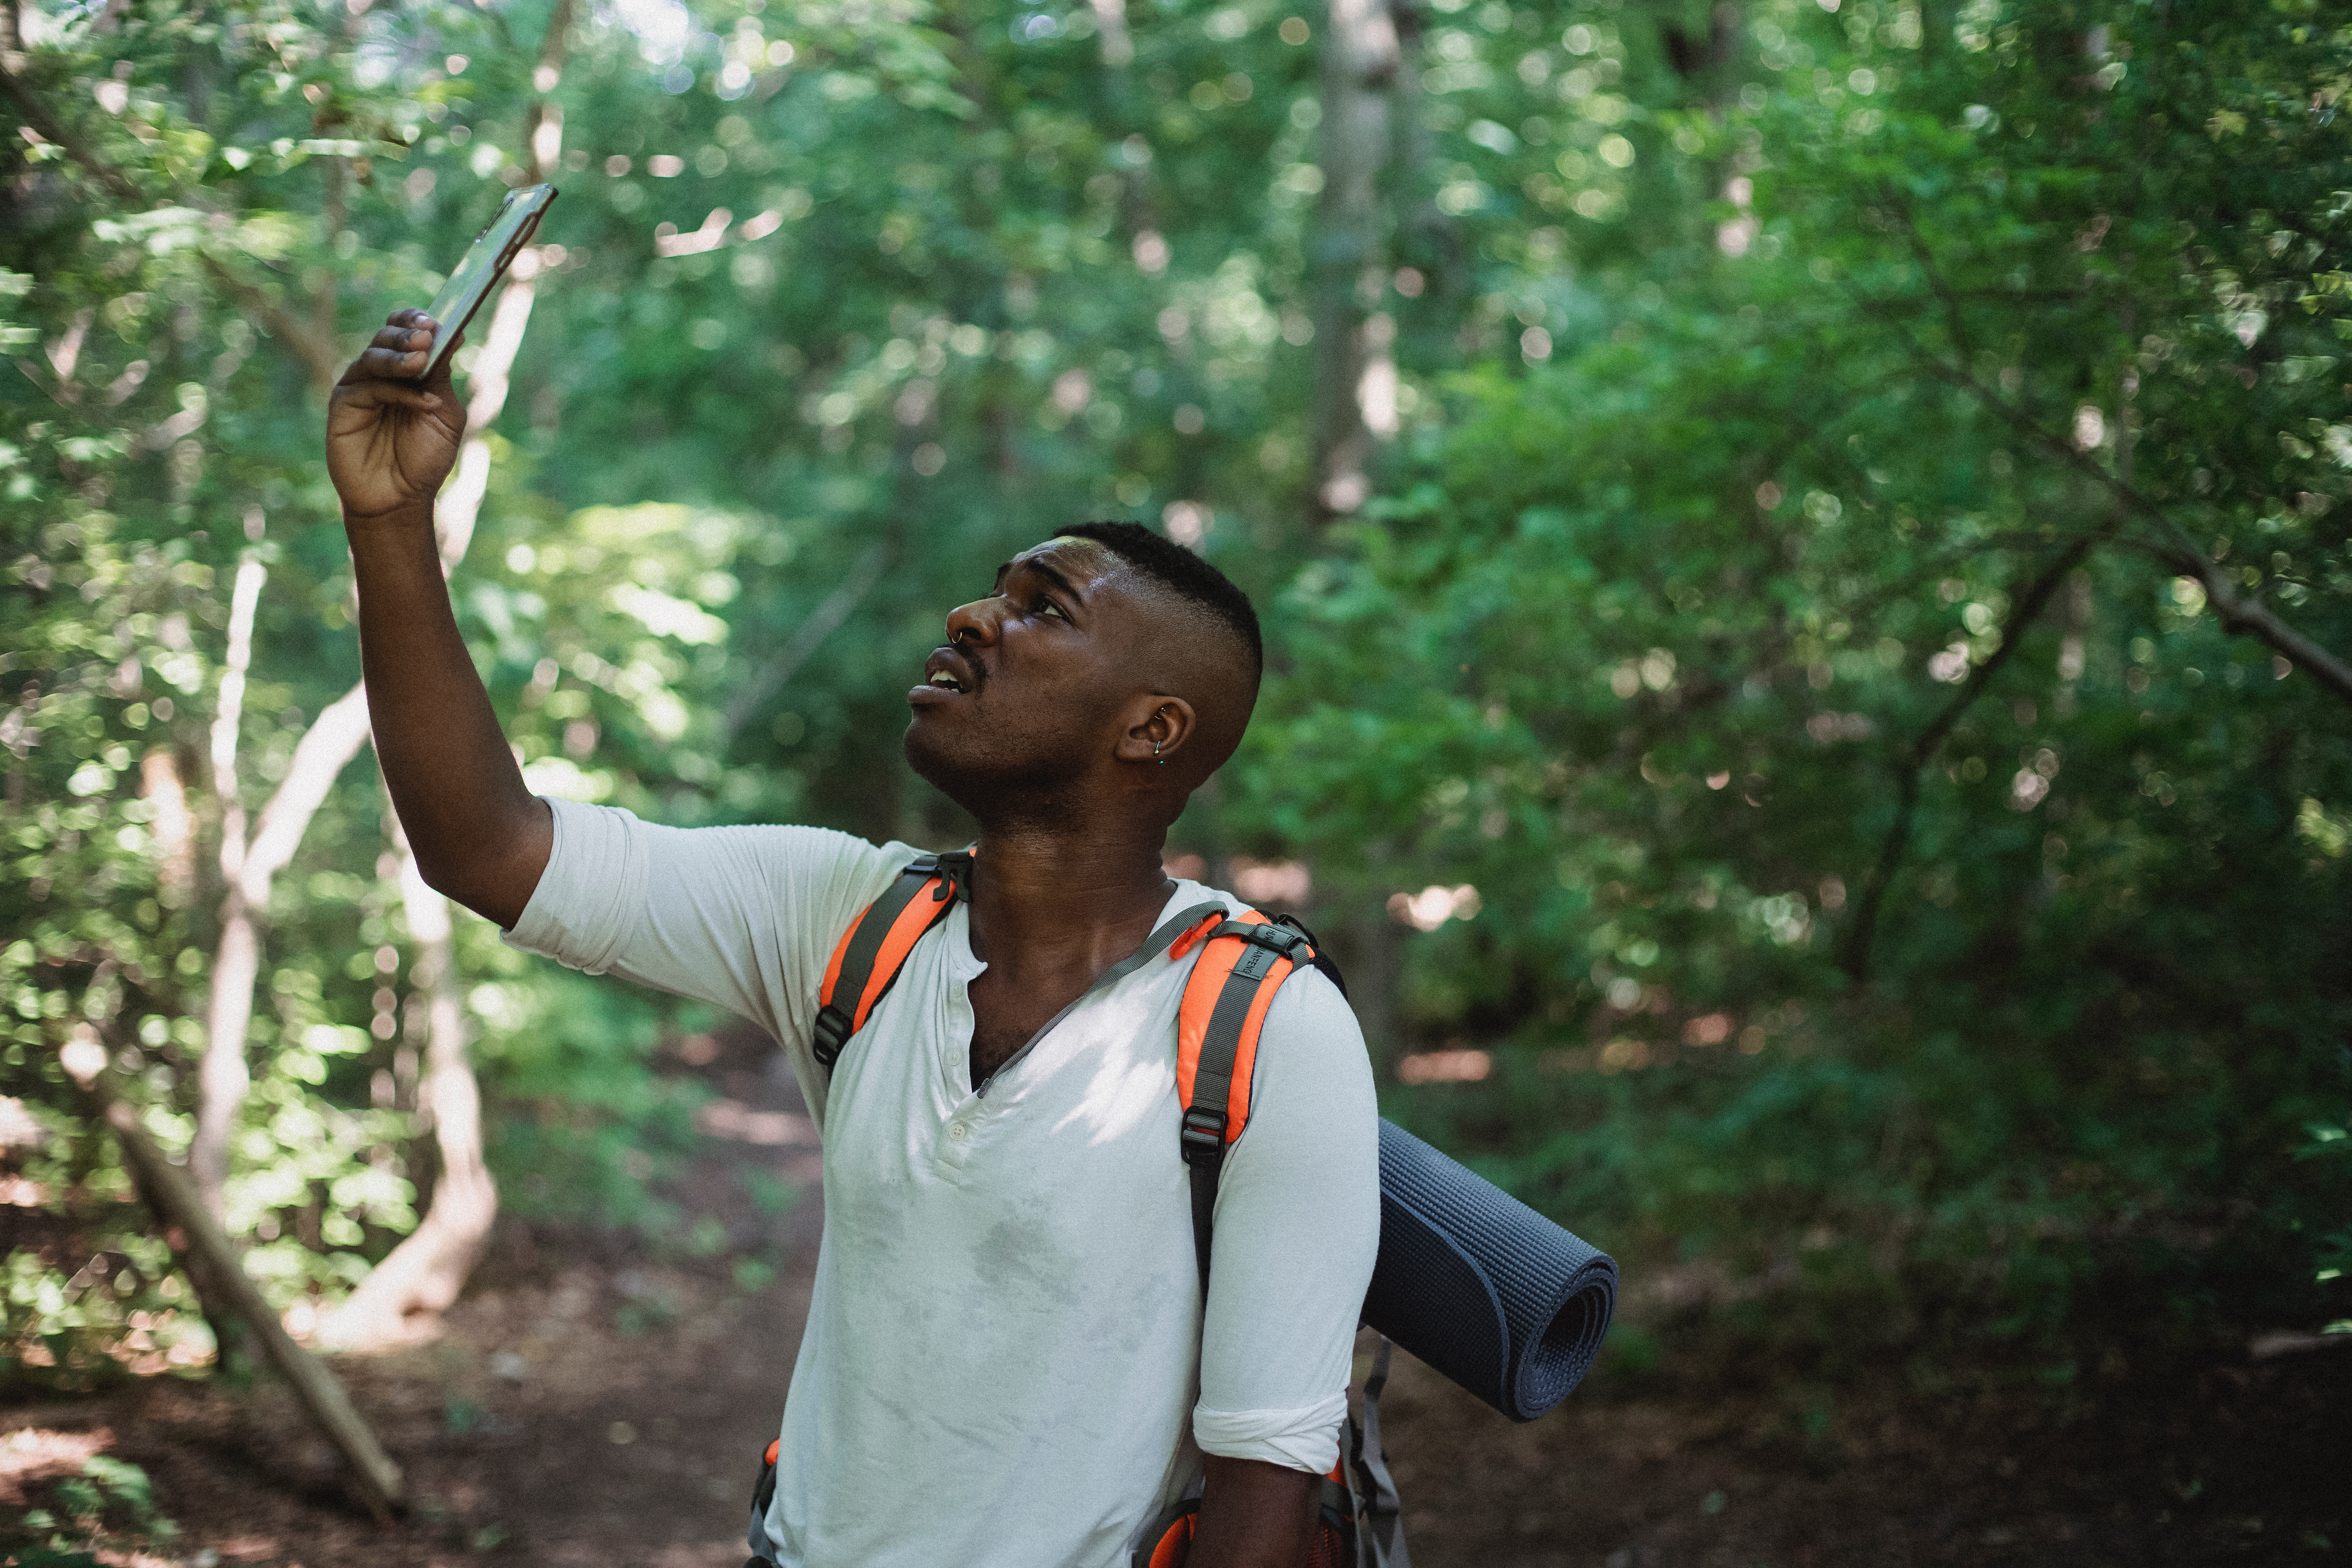
\includegraphics[width=0.6\textwidth]{media/no_internet.jpg}
	\end{figure}
\end{frame}
\begin{frame}   
	\frametitle{Situation 2: low battery}
	 \begin{figure}
		\centering
		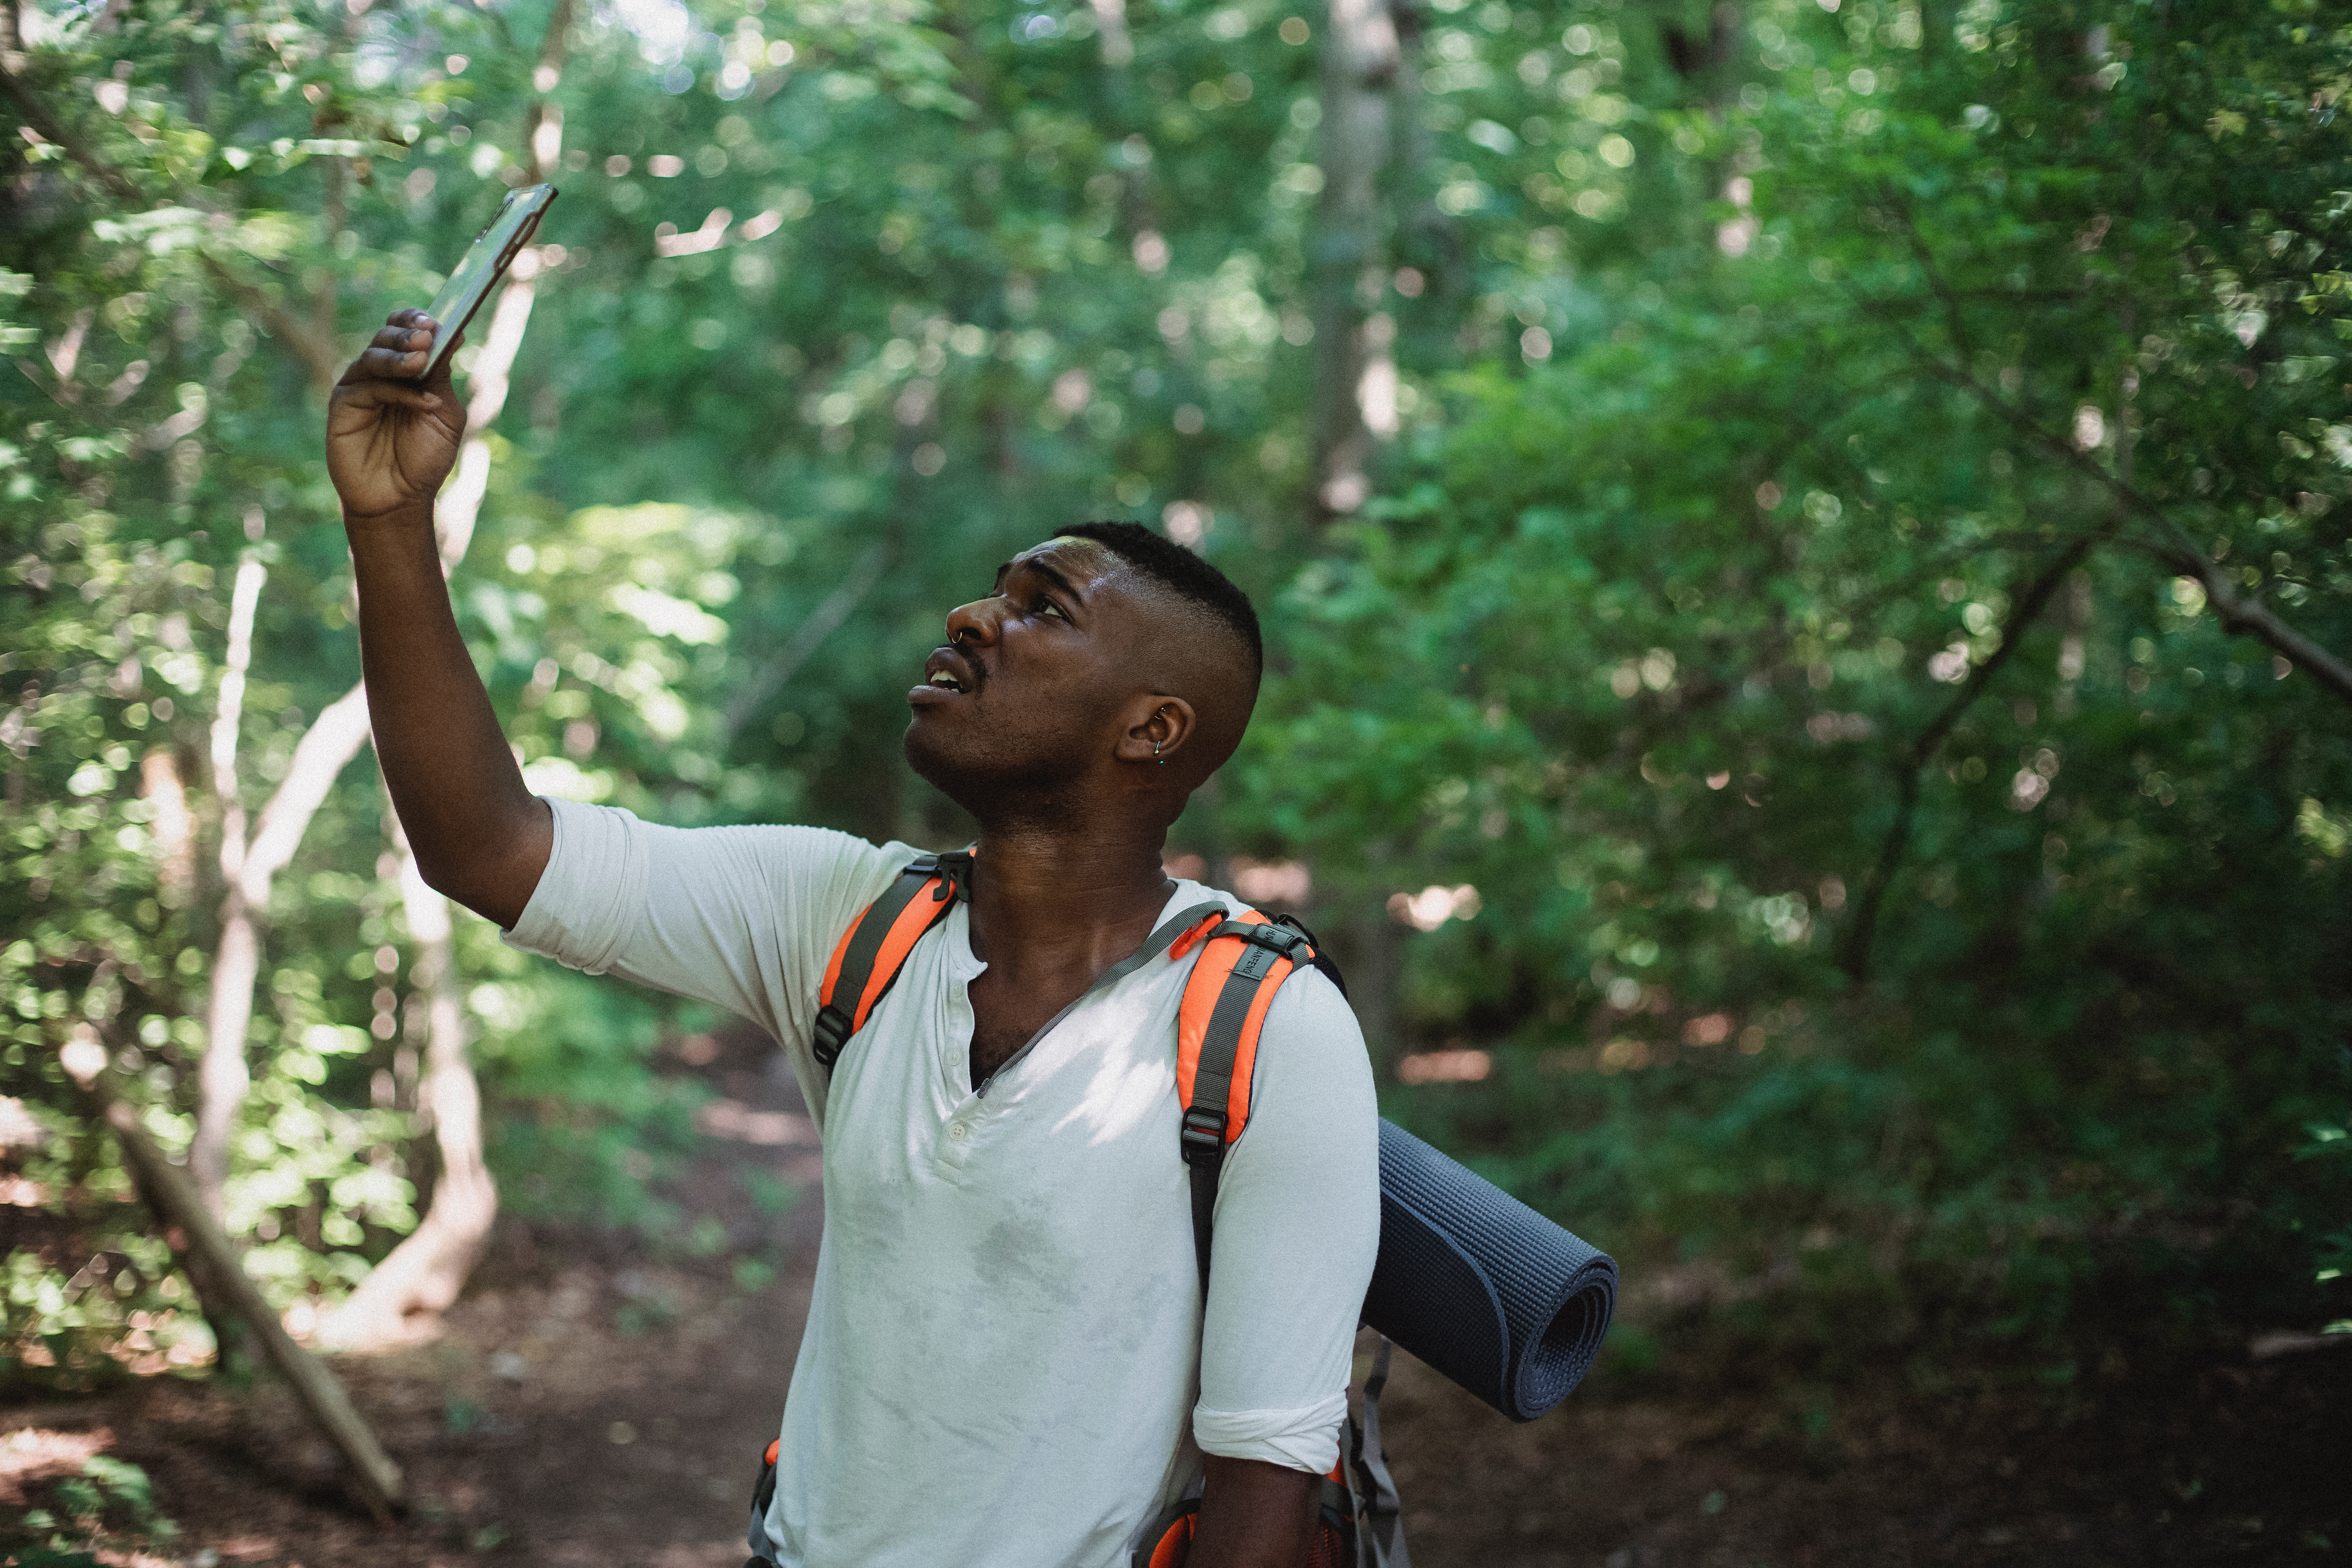
\includegraphics[width=0.6\textwidth]{media/no_internet.jpg}
	\end{figure}
\end{frame}




\section{Context Features}
\begin{frame}   
	\frametitle{Context features to control our adaptation}
	\begin{itemize}
		\item lokale SQL database
		\item small and lightweight json get and post requests?
		\item find efficient way to listen for new events
	\end{itemize}
\end{frame}




\section{Adaptation Mechanisms}
\begin{frame}   
	\frametitle{Adaptation Mechanisms}
	\begin{itemize}
		\item Adapt Data Transfer, instead of sending complete information, only send necessary parts, lazy evaluation of data
		\item Store events you participate in locally, create event hash for synchronization (should be smaller than complete object, however, it will interfere with energy challenge to some degree (complexe calculation <-> less data to transfer) 
	\end{itemize}
\end{frame}




\section{MAPE-K}
\begin{frame}   
	\frametitle{MAPE-K}
	\begin{itemize}
		\item Monitor - Sensor Data (of gps and internet connection) only when needed, limited background processes
    		\item Analyze - check event information like time and day 
    		\item Plan - if current\_time + threshold >= event\_time => check for updates on event
    		\item Execute - ask server for new hash of event -> if same, do nothing, else fetch data again
    		\item Knowledge - store personal and event information locally
	\end{itemize}
\end{frame}




\section{Detailed Architecture and Technology Choice}
\begin{frame}
	\frametitle{Detailed architecture and technology choice}
	 \begin{figure}
		\centering
		\includegraphics[width=0.6\textwidth]{media/architecture.jpg}
	\end{figure}
\end{frame}



\end{document}